\documentclass{article}
\usepackage{amsmath}
\usepackage{amsthm}
\usepackage{amsfonts}
\usepackage{amssymb}
\usepackage{bbold}
\usepackage{dsfont}
\usepackage{graphicx}
\usepackage{cleveref}
\usepackage{bm}
\usepackage{booktabs}
\usepackage{siunitx}
\usepackage{xcolor}
\usepackage{pdfpages}
\usepackage[utf8]{inputenc}
\usepackage[english]{babel}
\newtheorem{definition}{Definition}
\newtheorem{example}{Example}
\newcommand{\exP}[1]{\mathrm{e}^{#1}}
\newcommand{\dif}{\mathrm{d}}
\renewcommand{\vec}[1]{\mathbf{#1}}
\newcommand{\pdagger}{{\phantom{\dagger}}}
\newcommand{\state}[1]{\vert #1\rangle}
\newcommand{\cstate}[1]{\langle #1\vert}
\newcommand{\tr}[1]{\mathrm{tr}\left\{#1\right\}}
\newcommand{\trs}[2]{\, \mathrm{tr}_{#1}\{#2\}}
\newcommand{\expc}[3]{\langle #1\vert #2 \vert #3\rangle}
\usepackage[doi=false,url=false,isbn=false,backend=bibtex,style=nature,natbib=true,sorting=none]{biblatex}
\bibliography{bib.bib}
\usepackage{geometry}
\geometry{
	a4paper,
	total={170mm,257mm},
	left=15mm,
	right=15mm,
	top=15mm,
}
\begin{document}
\title{Report 25: TTHEOM results}
\maketitle

\begin{figure}[!h]
	\centering
	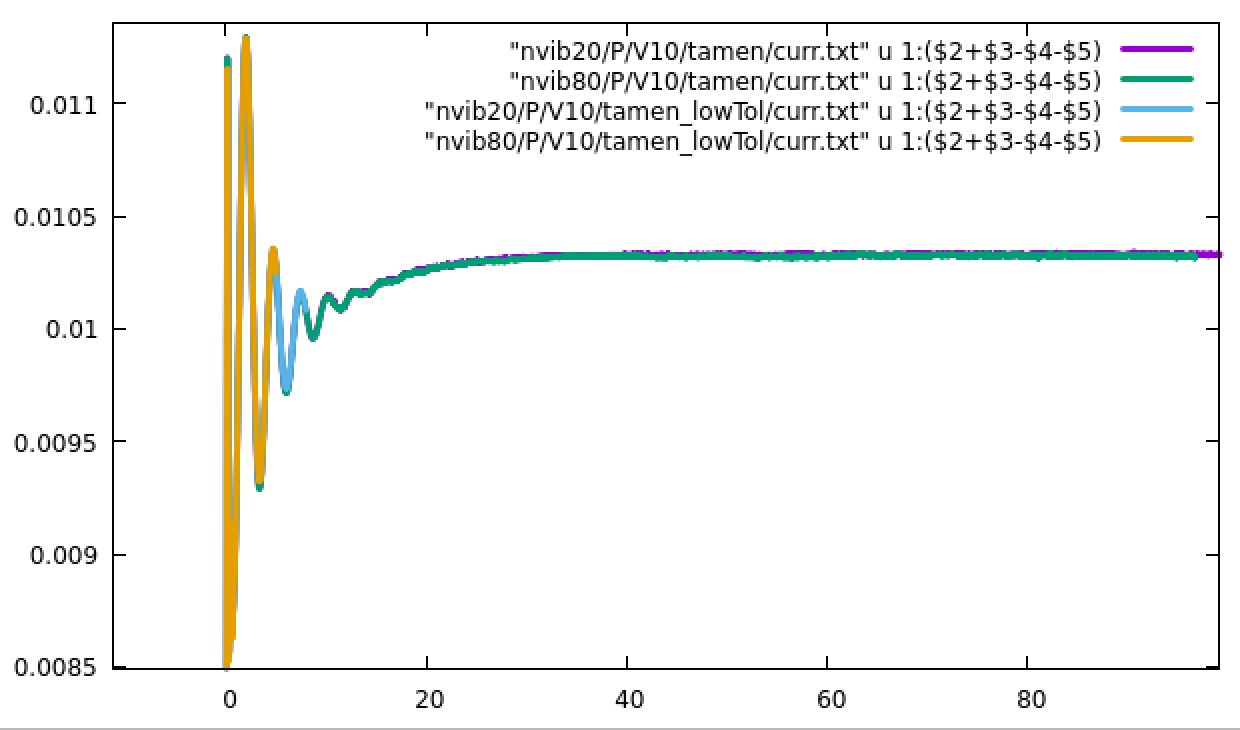
\includegraphics[width=0.5\textwidth]{figs/fig1.png}
	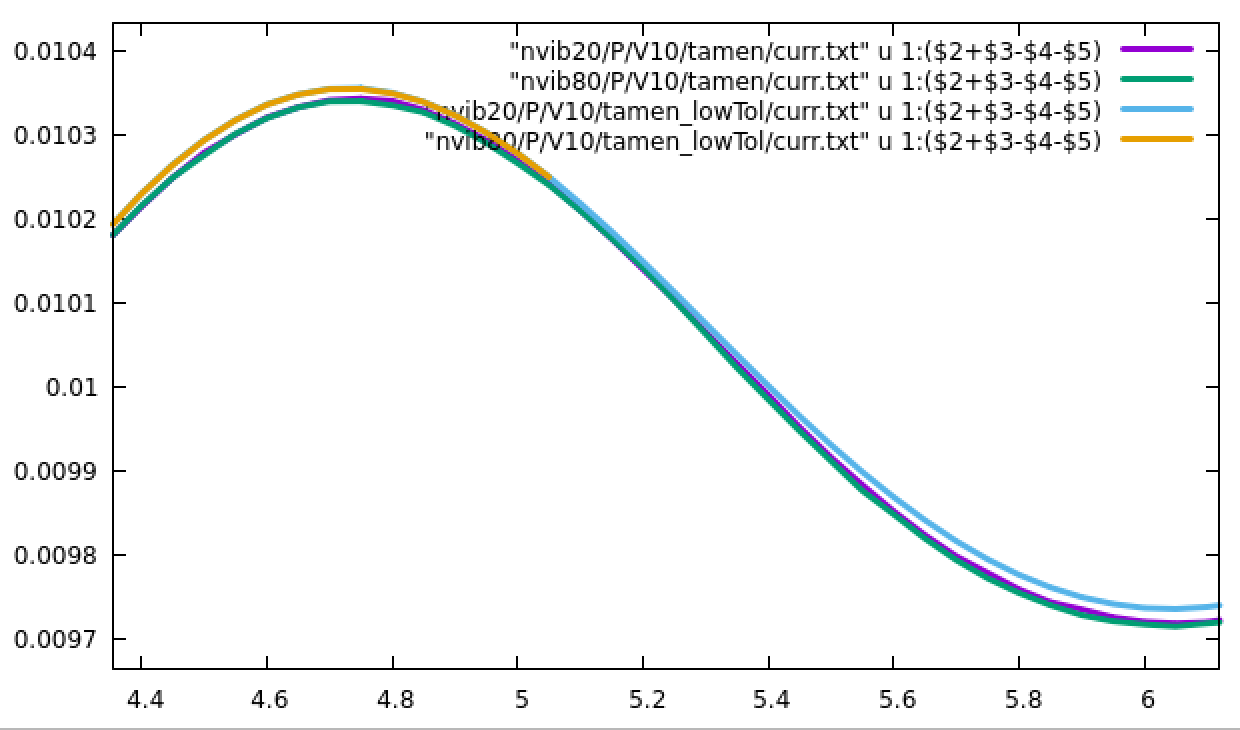
\includegraphics[width=0.5\textwidth]{figs/fig2.png}
	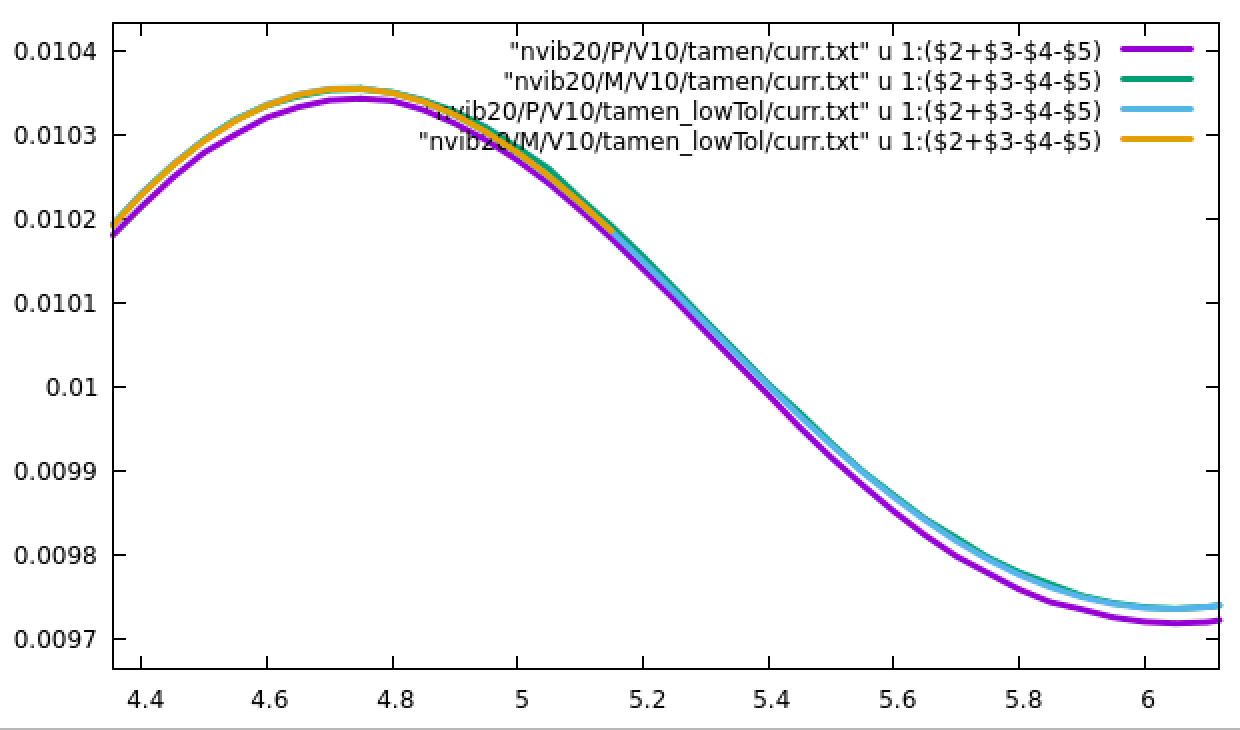
\includegraphics[width=0.5\textwidth]{figs/fig3.png}
	\caption{Charge current for $P=\frac{1}{2}$, $V=\SI{0.5}{\volt}$, varying $n_\mathrm{vib}$ for tolerances tol$\ = 10^{-3}$ (purple, green), and tol$\ = 10^{-4}$ (blue, yellow) (top and middle panel); comparison of charge currents for $A=\frac{1}{2}$ and $A=-\frac{1}{2}$ (bottom panel). This plot shows that for a higher tolerance, it appears that the vibrational basis is not converged. This is not true, because when decreasing the error tolerance, no difference for $n_\mathrm{vib}=20$ and $n_\mathrm{vib}=80$ is observed. The difference in charge currents for opposing lead magnetizations (for a low tolerance) is as large as the change in the current when decreasing the tolerance.}
\end{figure}
\begin{figure}[!h]
	\centering
	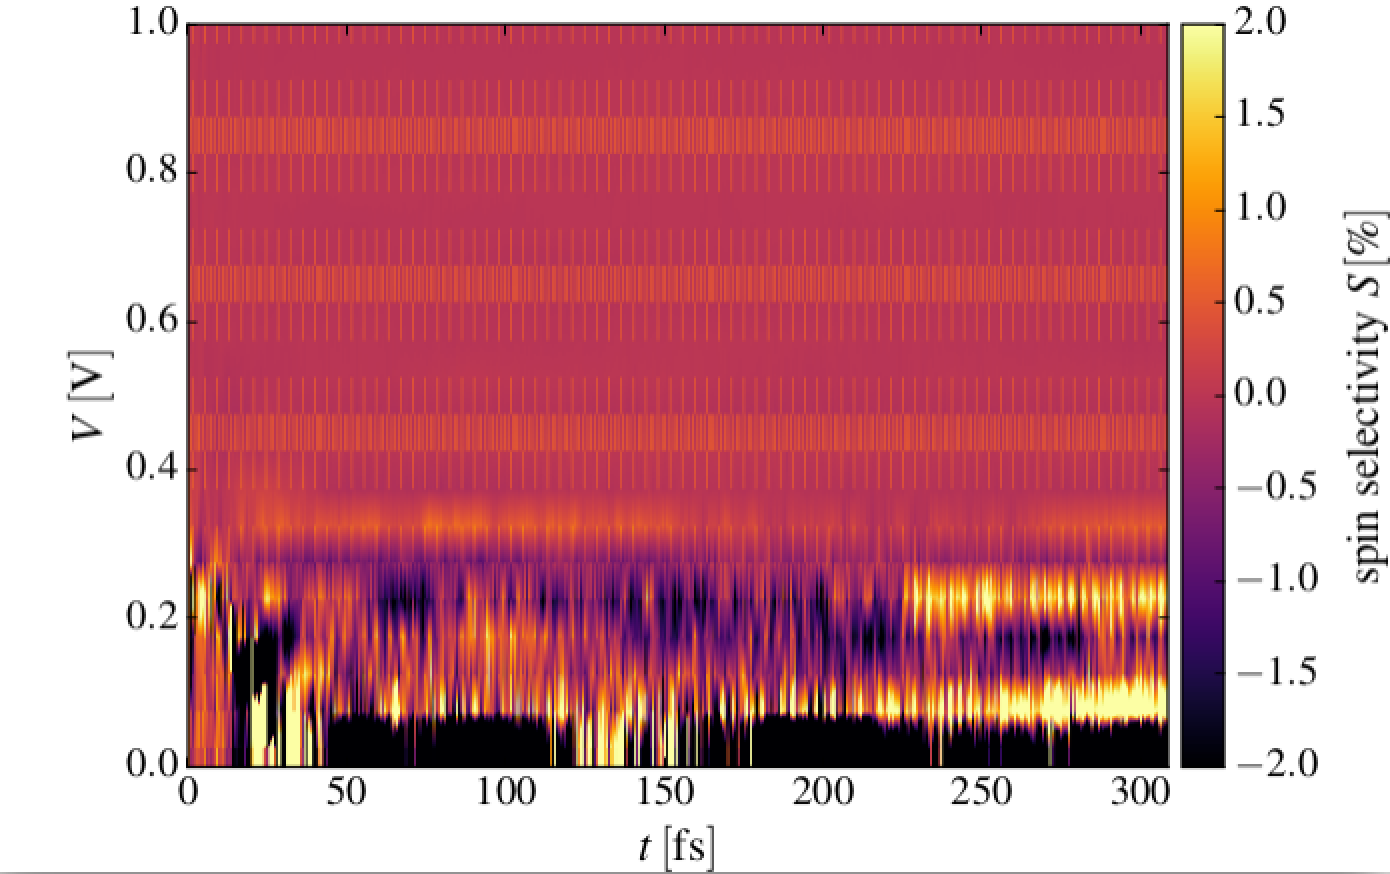
\includegraphics[width=0.6\textwidth]{figs/fig4a.png}
	\caption{$n_\mathrm{vib}=20$, tol$\ =10^{-3}$}
\end{figure}
\begin{figure}[!h]
	\centering
	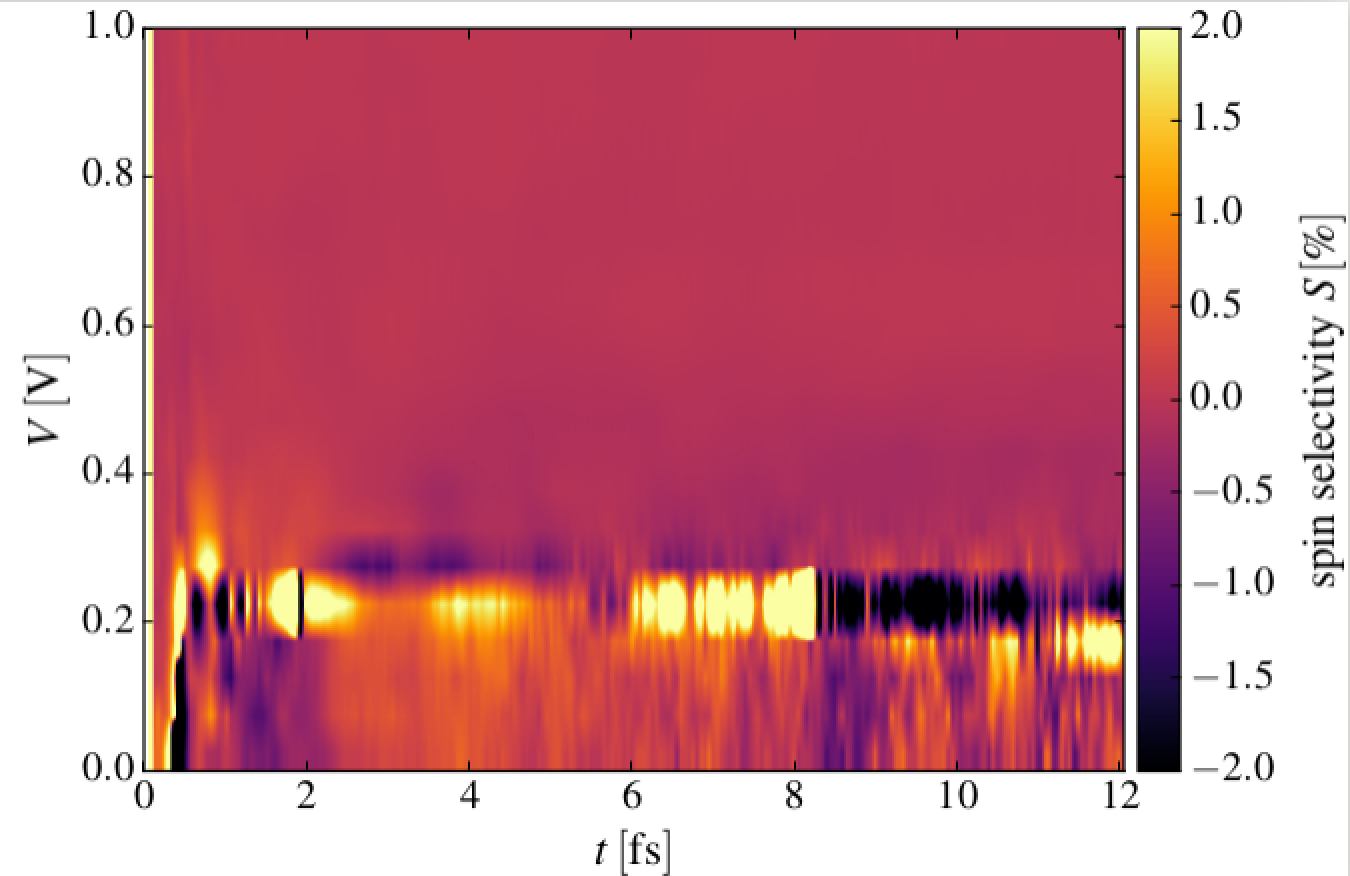
\includegraphics[width=0.6\textwidth]{figs/fig4b.png}
	\caption{$n_\mathrm{vib}=20$, tol$\ =5\cdot 10^{-4}$}
\end{figure}
\begin{figure}[!h]
\centering
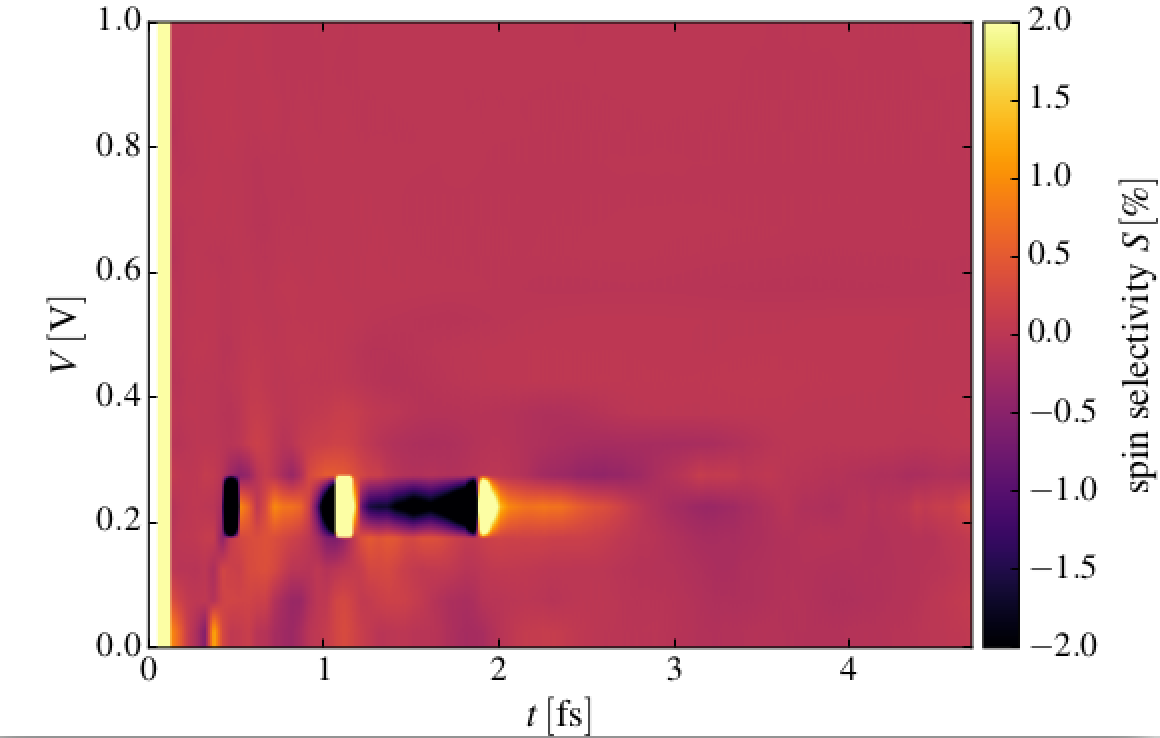
\includegraphics[width=0.6\textwidth]{figs/fig4c.png}
\caption{$n_\mathrm{vib}=20$, tol$\ =10^{-4}$. Features, that can be seen in the upper plot for $V<\SI{0.2}{\volt}$ dissapear entirely when decreasing the error tolerance.}
\end{figure}
\begin{figure}[!h]
	\centering
	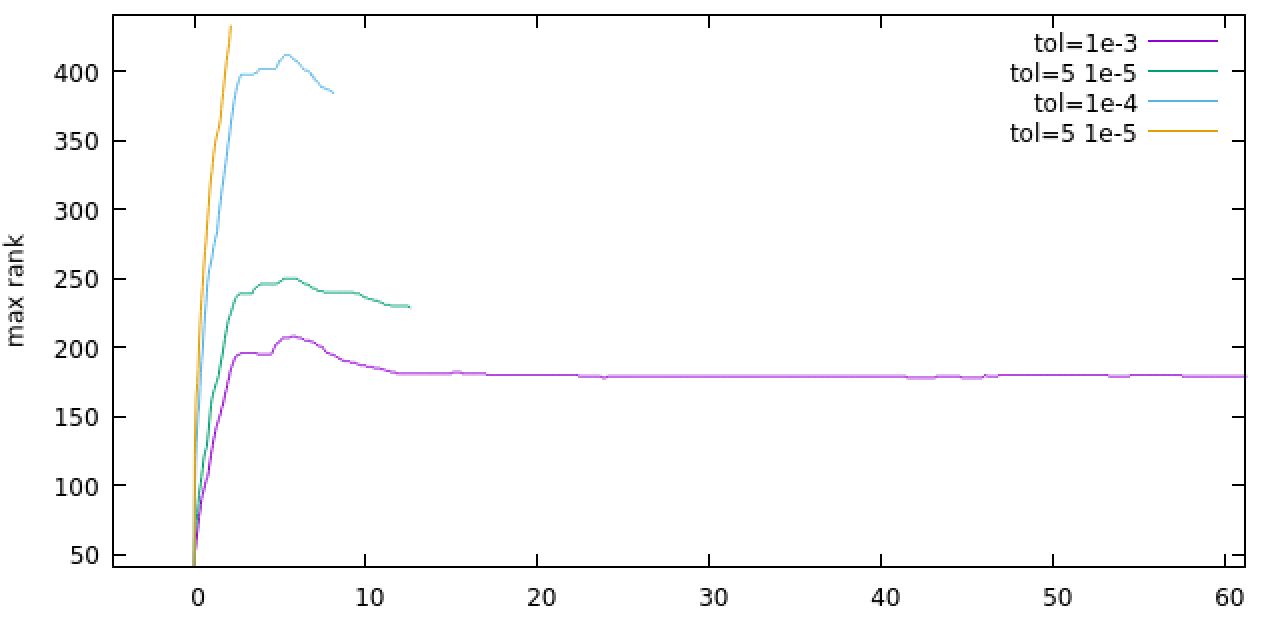
\includegraphics[width=0.8\textwidth]{figs/fig5.png}
	\caption{Maximal rank of tensor train for $V=\SI{0.5}{\volt}$, $n_\mathrm{vib}=20$. }
\end{figure}


\end{document}


